\documentclass[main.tex]{subfiles} 
\begin{document}

\section{Mangfold i naturen}
Ved endt opplæring skal eleven kunne
\begin{itemize}[noitemsep]
\item forklare hovedtrekkene i evolusjonsteorien og gjøre rede for observasjoner som støtter teorien
\item beskrive oppbygningen av dyre- og planteceller og forklare hovedtrekkene i fotosyntese og celleånding
\item gjøre rede for celledeling og for genetisk variasjon og arv
\item forklare hovedtrekk i teorier for hvordan jorda endrer seg og har endret seg gjennom tidene, og grunnlaget for disse teoriene
\item undersøke og registrere biotiske og abiotiske faktorer i et økosystem i nærområdet og forklare sammenhenger mellom faktorene
\item observere og gi eksempler på hvordan menneskelig aktivitet har påvirket et naturområde, undersøke ulike interessegruppers syn på påvirkningen og foreslå tiltak som kan verne naturen for framtidige generasjoner
\item gi varierte eksempler på hvordan samer utnytter ressurser i naturen
\end{itemize}

\subsection{Evolusjonsteorien}
{\color{Blue}Forklare og gjøre rede for - middelskompetansenivå}
\newline\newline
Evolsjonsteorien er en vitenskapelig teori som forklarer og predikerer naturlige fenomener. Frem til 19 århundre, var det antatt at arter forble uforandret siden de ble skapt. Forskningen til Charles Darwin banet veien for dagens forståelse, der arter kan forandres gjennom \emph{naturlig og kunstig seleksjon}, og ved å \emph{tilpasse} seg til sine omgivelser.
\newline\newline
Mennesker har over mange generasjoner utvalgt og oppdrett ønskede egenskaper, gjennom prosessen som kalles \textbf{kunstig seleksjon}. Darwin argumenterte at en tilsvarende prosess forekommer i naturen. \textbf{Naturlig seleksjon} er en prosess der individer som har visse arvelige egenskaper overlever og reproduserer ved et høyere andel enn andre individer på grunn av disse egenskapene. Over tid kan naturlig seleksjon øke organismens tilpasningsevne til deres omgivelser. Hvis omgivelsene og miljøet forandrer, eller individer flytter til en ny omgivelse, naturlig seleksjon kan resultere i tilpasning til disse nye omgivelsene, som noen ganger gir \textbf{opphav} til nye arter.
\newline\newline
Alle levende organismer er utsatt for konkurranse for ressurser, men også predasjon\footnote{Predasjon, defineres bredt som at en organisme spiser hele eller deler av en annen organisme.}. Naturlig seleksjon forekommer ofte ved interaksjon av organismer med andre organismer, så vel som interkasjon av orgranismer med deres fysiske omgivelser.
\newline\newline
Blant direkte observasjoner av evolusjonære forandringer er insekten Serinethinae (eng.: Soapberry bug). I et studie \cite{cabo92}, ble fremvist at insektens ``nebb'' ble lengere når den måtte forandre sine spisevaner. En pågående eksempel på naturlig seleksjon som har en stor dramatisk påvirkning på mennesker er evolusjon av antibiotika resistente bakterier. En annen type bevis for evolusjon kommer fra analysering av likheter mellom forskjellige organismer. 


%\pagebreak[4]\global\pdfpageattr\expandafter{\the\pdfpageattr/Rotate 270}
\begin{sidewaysfigure}
    \label{fig:evolusjon}
    \centering
    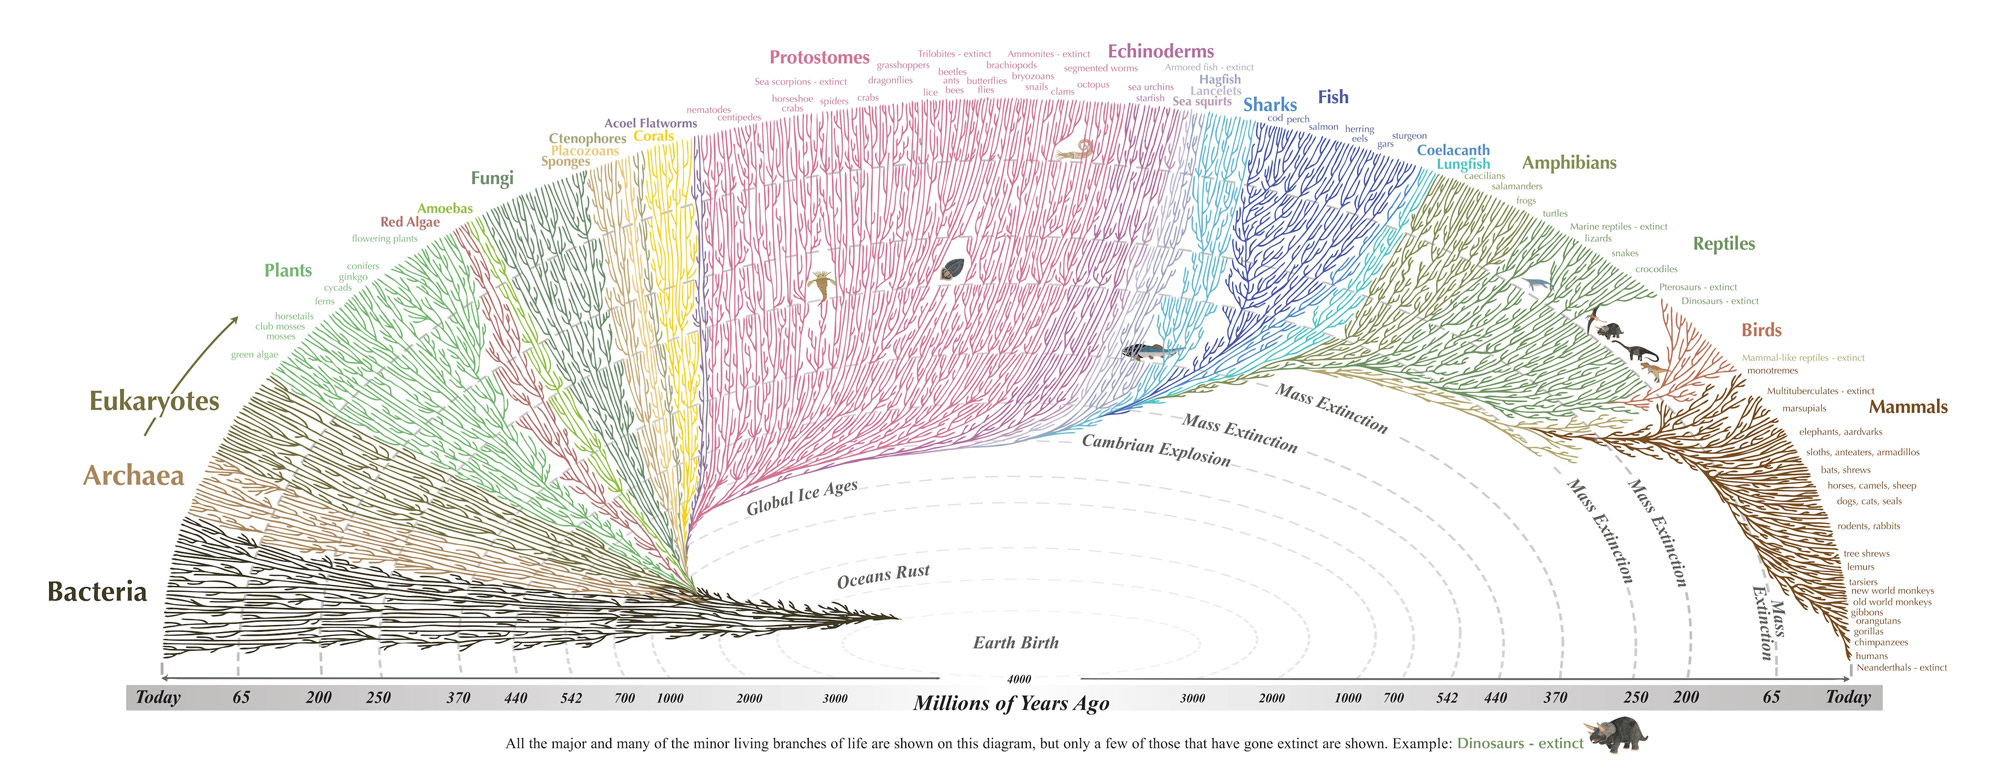
\includegraphics[width=1.1\textwidth,left]{../figures/utviklingavliv.jpg}
    \caption{Utvikling av liv og forbindelsene mellom arter. Kilde: evogeneao.com}
\end{sidewaysfigure}

\newpage
\hspace{-6mm}En tredje type bevis for evolusjon er fossiler \footnote{Bevarte rester eller spor av organismer fra fjern fortid.}. Bevarte fossiler dokumenterer et mønster av evolusjon, som viser at tidligere organismer var forskjellige fra dagens organismer and at mange arter har utdødd.
\newline\newline
En forståelse for evolusjon gir oss en nærmere tilknytning til resten av skapninger på jorden, hvor vi alle er lenket sammen gjennom jordens utvikling og utforming (se figur \ref{fig:evolusjon}).

\subsection{Celler og oppbygging av celler}
{\color{PineGreen}Beskrive - lavt kompetansenivå}
\newline\newline
Alle organismer består av celler. Akkurat slik atomer er grunnleggende i kjemi, er celler på tilsvarende vis i biologi. De enkleste levende organismer er enkelt cellede organismer, mens vi mennesker og andre komplekse organismer er flercellede organismer. En oversikt over celleoppbygging er gitt i figur \ref{fig:celler}.
\newline\newline
\textbf{Cellemembranen} huser cellens indre membraner, som er detaljert arrangert og deler cellen i flere kamre, også kalt \emph{organeller}.
\newline\newline
\textbf{Cellekjernen} har blant annet \textbf{kromosomer}, som besitter gener i form av \textbf{DNA}.
\newline\newline
\textbf{Cellevegg} finnes hos noen type celler utenfor cellemembranen og gir beskyttelse til cellen, og også som en filtrerings mekanisme. Finnes ofte hos planter og alger, men ikke dyr.
\begin{figure}[h!]
\centering
    \begin{subfigure}{.5\textwidth}
    \centering
    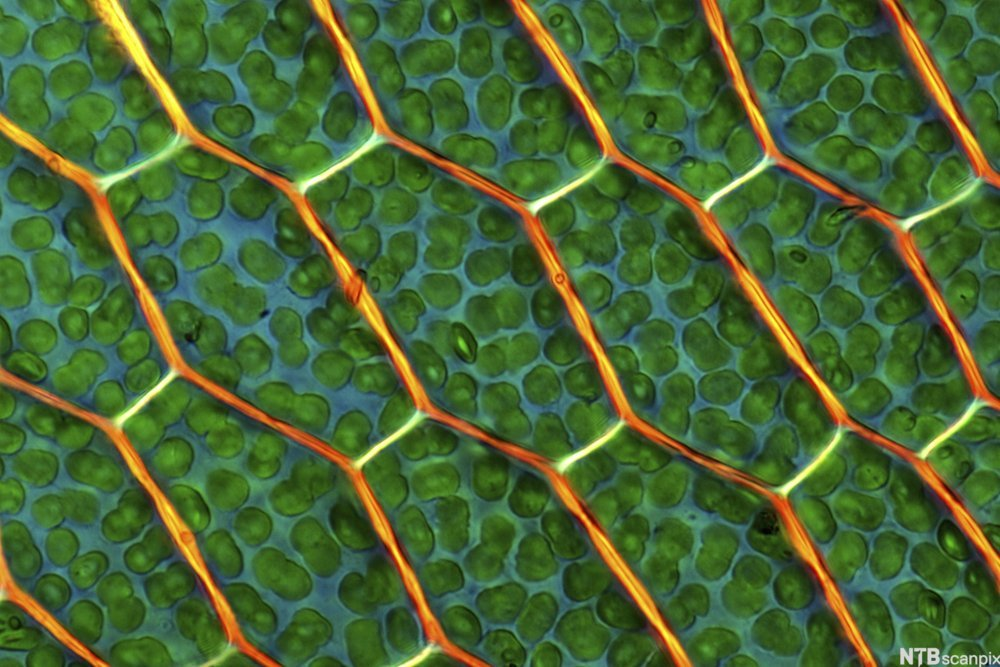
\includegraphics[scale = 0.5]{../figures/cellevegg.jpg}
    \caption{Moseceller med tydelige cellevegger. Celleorganellet kloroplast er også synlig. Kilde: Ndla}
    \end{subfigure}%%
    \begin{subfigure}{.5\textwidth}
    \centering
    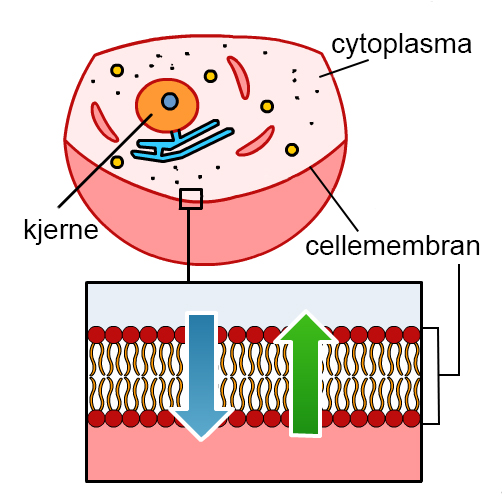
\includegraphics[scale = 0.25]{../figures/cellemembran.jpg}
    \caption{En dyrecelle. Kilde: Ndla}
    \end{subfigure}
    \begin{subfigure}{.5\textwidth}
    \centering
    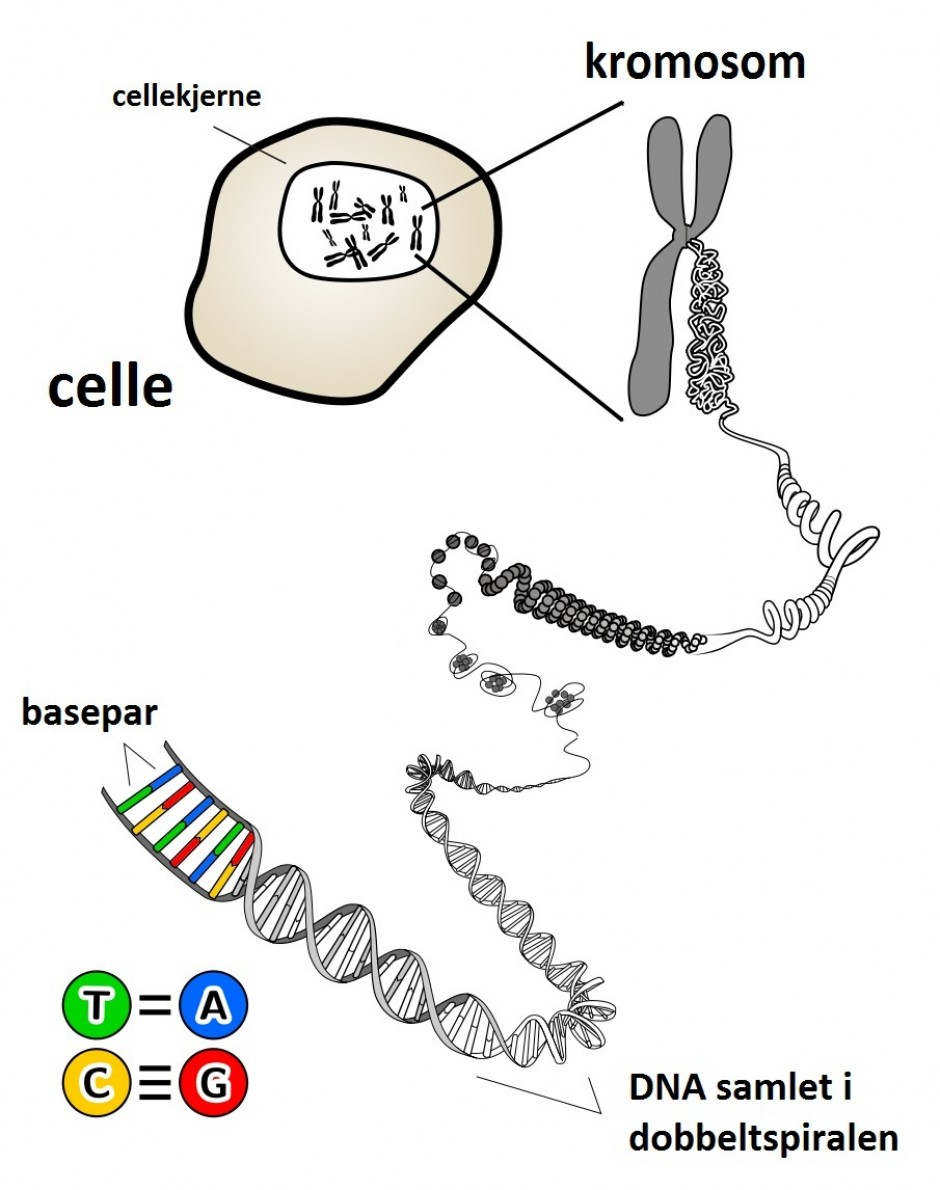
\includegraphics[scale = 0.20]{../figures/dna.jpg}
    \caption{Kromosom i cellekjernen. Kilde: forskning.no}
    \end{subfigure}
    \caption{Oppbygging av celler}
    \label{fig:celler}
\end{figure}

\subsection{Celledeling}
{\color{Blue}Forklare og gjøre rede for - middelskompetansenivå}
\newline\newline

\subsection{Celleånding}
{\color{Blue}Forklare og gjøre rede for - middelskompetansenivå}
\newline\newline
Levende celler er avhengig av energi for å kunne utføre cellens funksjoner, deriblant å kunne forflytte seg og reprodusere. En ku får i seg energi ved å beite på gress; mens andre organismer får i seg energi ved å spise andre dyr som spiser planter. Energien som lagres i mat kommer opprinnelig fra solen. Energi strømmer inn i et økosystem som sollys og går ut som varme; i motsetning, de kjemiske elementene som er essensielle for liv blir resirkulert. Fotosyntese generer oksygen og organiske molekyler som brukes av mitokondrier\footnote{En organell som finnes i de fleste celler, der de biokjemiske prosessene for celleånding og energi produksjon forekommer.} som brensel for \textbf{celleånding}. Avfallsproduktet fra celleåndingen er karbondioksid og vann, som igjen brukes i fotosyntese. Denne prosessen kan oppsummeres som følgende:
\begin{align*}
\text{Organisk materie} + \text{Oksygen} \longrightarrow \text{Karbondioksid} + \text{Vann} + \text{Energi}
\end{align*}
Et spesifikk eksempel på celleånding er \textbf{oksidering}\footnote{
    Når en elektron binder seg til et atom eller løsriver seg fra et atom, blir energi, som er lagret i organiske molekyler sluppet, og denne energien brukes av celler for å f.eks forflytte seg eller reprodusere. I mange kjemiske reaksjoner forekommer det overføring av en eller flere elektroner ($e^{-1}$) fra en reaktant. Disse elektronoverføringene kalles \emph{redoksreasksjon}. I en redoksreaksjon, tap av elektroner fra et stoff kalles oksidering, og tilegnelse av elektroner til et annen stoff kalles reduksjon. Et enkel (ikke-biologsik) eksempel er reaksjonen mellom natrium (Na) og klor (Cl) som danner bord salt: 
    \begin{align*} 
        \text{Na} + \text{Cl} \longrightarrow \text{Na}^+ + \text{Cl}^-
    \end{align*}} 
av \emph{monosakkariden glukose} ($\text{C}_6 \text{H}_{12} \text{O}_6$):
\begin{align}
\label{celleånding}
\text{C}_6\, \text{H}_{12}\, \text{O}_6 + 6\, \text{O}_2 \longrightarrow 6\, \text{CO}_2 + 6\, \text{H}_2\, \text{O} + \text{Energi}
\end{align}
Cellen bryter ned glukosen og andre organiske brennstoff for å produsere kjemisk energi. I \emph{aerobisk ånding} benyttes oksygen som en reaktant. Energien i mat molekyler tapes av cellen gjennom reduksreaksjoner, der et stoff delvis eller helt overfører elektroner til et annet stoff.

\subsection{Fotosyntese}
{\color{Blue}Forklare og gjøre rede for - middelskompetansenivå}
\newline\newline
Kloroplast i planter fanger sollys som har reist cirka 150 millioner kilometer fra solen og konverterer den til kjemisk energi som deretter blir lagret i sukker og andre organiske molekyler. Hele denne prosessen kalles \textbf{fotosyntese}.
\newline\newline
Fotosyntesen forer nesten hele den levende verden, enten direkte eller indirekte. En organisme tilegner seg energi gjennom en av to hoved modus: \emph{autotrof} eller \emph{heterotrof}. Nesten alle planter regnes som autotrofe siden de kan leve og formere seg utelukkende ved uorganisk ernærning (vann, salter og karbondioksid). Planter blir referert som \emph{fotoautotrofer}, organismer som benytter lys som kilde til energi til å lage organiske stoffer. Autotrofer er den ultimate kilden for organiske stoffer for alle ikke-autotrofe organismer, og for denne grunn, biologer referer til autotrofer som produsenter av biosfæren\footnote{Delen av atmosfæren hvor liv eksisterer.}. Hetrotrofer tilegner seg næring gjennom den andre hoved modus. Ute av stand til å lage egen mat, de lever på stoffer produsert av andre orgranismer (hetro- betry ``andre''). Hetrotrofer er biosfærens konsumenter.
\newline\newline
Alle grønne deler av en plante, inkludert grønne stilker og umoden frukt, har \textbf{kloroplaster}, men bladene er hoved kilden til fotosyntese i de fleste planter. Karbondioksid trer inn i bladet, og okysgen forlater, gjennom mikroskopiske porer (så-kalte spalteåpninger). \textbf{Klorofyll}, den grønne pigmentasjonen som gir blader deres farge, absorberer sollys som igjen driver prosessen av dannelsen av organiske molekyler i kloroplasten. Vi kan oppsummere den complekse serie med kjemiske reaksjoner i fotosyntese med følgende kjemisk ligning:
\begin{align*}
6\,\text{CO}_2 + 12\,\text{H}_2\,\text{O} + \text{Lys energi} \longrightarrow \text{C}_6\,\text{H}_{12}\,\text{O}_6 + 6\,\text{O}_2 + 6\,\text{H}_2\,\text{O}
\end{align*}
Forenklet kan dette skrives,
\begin{align}
\label{fotosyntese}
6\,\text{CO}_2 + 6\,\text{H}_2\,\text{O} + \text{Lys energi} \longrightarrow \text{C}_6\,\text{H}_{12}\,\text{O}_6 + 6\,\text{O}_2
\end{align}
Vi kan se at den kjemiske forandringen gjennom fotosyntesen er den motsatte av den som forekommer gjennom celleånding (se ligning: \ref{celleånding}).

\subsection{Jordens utvikling}
{\color{Blue}Forklare - middelskompetansenivå}
\newline\newline
Jorda er en planet i kontinuerlig forandring. Sidens dens formasjon (mao. dannelse), dvs. \textbf{4.6 milliarder år} siden, har planeten gått gjennom flere geologiske epoker. Under formasjonen av planeten, ble de tyngere metaller trukket mot sentrum av jorden og dannet \textbf{jordas kjerne}. Stoffer med mindre massetetthet dannet laget omkring kjernen og dette laget kalles \textbf{mantelen}. Over tid kjølnet det ytre laget til mantelen og dannet \textbf{jordskorpen}.
\begin{figure}[h!]
    \label{fig:evolusjon}
    \centering
    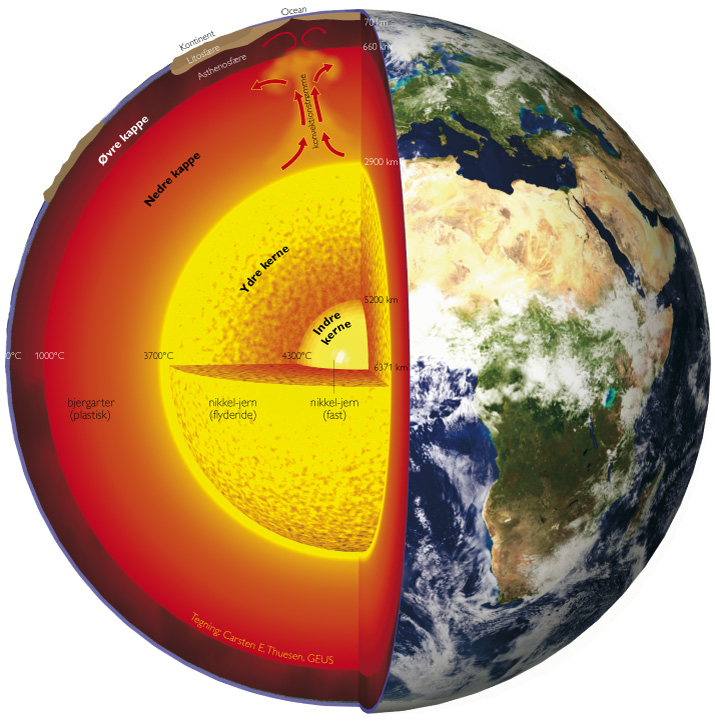
\includegraphics[scale = 0.7]{../figures/jordas_indre.jpg}
    \caption{Jordas indre. Kilde: www.geus.dk/}
\end{figure}

\subsection{Miljø og naturen}

\end{document}